\begin{fact} \label{exp-tab-var}
	La fonction $\exp$ admet le tableau de variations suivant.
	%
	\begin{center}
        \begin{tikzpicture}
            \tkzTabInit{
            	$x$      / 1 , 
				$\exp x$  / 1.5
			}{$0$, $+\infty$}

            \tkzTabVar{-/ {\small$0$}, +/ {\small$+\infty$}}
        \end{tikzpicture}
	\end{center}
\end{fact}


\begin{proof}
	Soient $\setproba{L}$ et $\setproba{E}$ les représentations graphiques respectives des fonctions $\ln$ et $\exp$, ainsi que $\Delta: y = x$.
	%
	\begin{itemize}
		\item La monotonie de $\exp$ découle de celle de $\ln$,
		et de la symétrie révélée dans le \reffact{exp-sym-ln}.
		%
		En effet,
		dans la figure suivante, nous partons de $a < b$.
		Comme $x(M) < x(N)$, nous avons $y(M^{\,\prime}) < y(N^{\,\prime})$ par symétrie.
		Il est immédiat de conclure.

		\begin{center}
			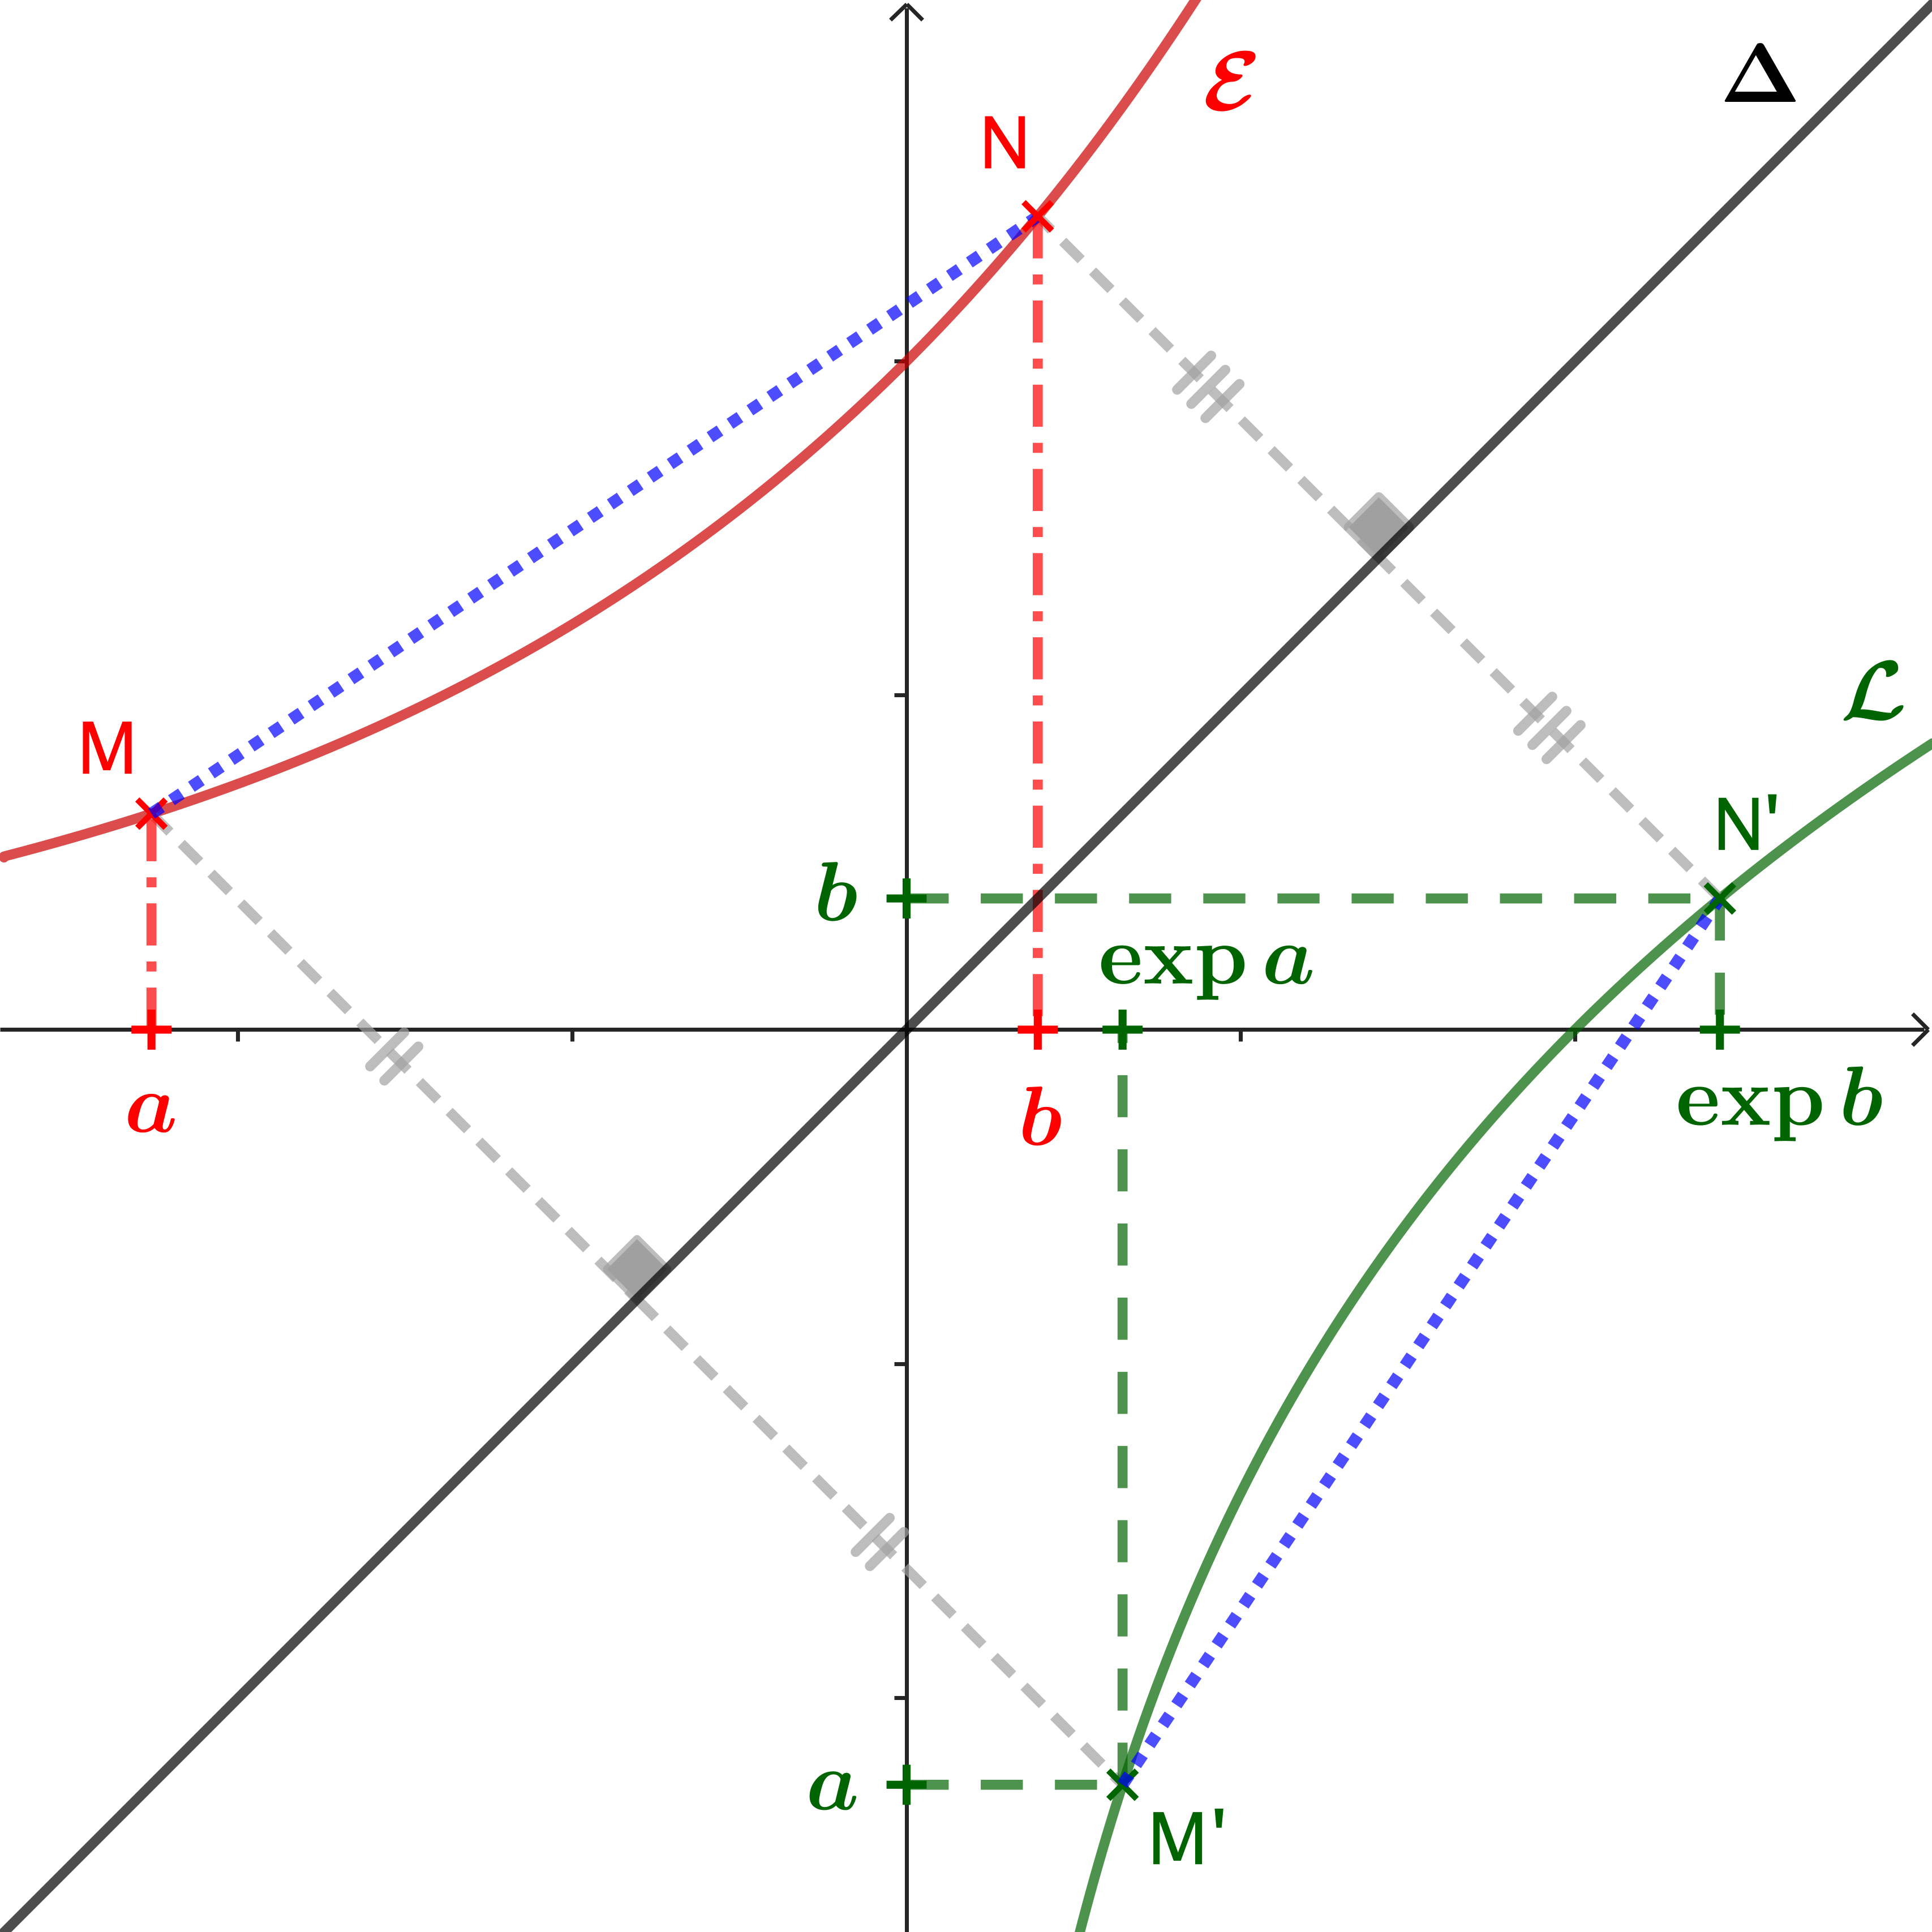
\includegraphics[scale=.55]{content/exp/monotony.png}
		\end{center}
	

		\item La limite en $+\infty$ découle rapidement de 
		$\exp(\ln(10^n)) = 10^n$,
		et de la stricte croissance de $\exp$ qui donne $\exp x > 10^n$ dès que $x > \ln(10^n)$.

		
		\item Pour la limite en $-\infty$, le plus efficace est de passer via $\exp(- x) = \frac{1}{\exp x}$ pour aboutir à
		$\limit{\exp x}{x}{-\infty} = \limit{\big( \frac{1}{\exp x} \big)}{x}{+ \infty}$.
		%
		On peut aussi le faire à la main via $\ln(10^{-n})$.
	\end{itemize}
\end{proof}

